% VUT FIT MITAI
% MSZ 2021/2022
% Author: Vladimir Dusek
% Login: xdusek27

%%%%%%%%%%%%%%%%%%%%%%%%%%%%%%%%%%%%%%%%%%%%%%%%%%%%%%%%%%%%%%%%%%%%%%%%%%%%%%%%

% Path to figures
\graphicspath{{tin/konecne_automaty/figures}}

%%%%%%%%%%%%%%%%%%%%%%%%%%%%%%%%%%%%%%%%%%%%%%%%%%%%%%%%%%%%%%%%%%%%%%%%%%%%%%%%

\chapter{TIN~--~Konečné automaty (jazyky přijímané KA, varianty KA, minimalizace KA, Mihill-Nerodova věta).}

% Todo:
% - Prevod RKA na DKA

%%%%%%%%%%%%%%%%%%%%%%%%%%%%%%%%%%%%%%%%%%%%%%%%%%%%%%%%%%%%%%%%%%%%%%%%%%%%%%%%

\section{Zdroje}

\begin{compactitem}
    \item \path{tin_2021_merged.pdf}
    \item \path{TIN_2020-09-22.mp4}
    \item \path{TIN_2020-09-29.mp4}
    \item \path{TIN_2020-10-02_demo.mp4}
    \item \path{TIN_2020-10-06.mp4}
    \item \path{TIN_2020-10-16_demo.mp4}
\end{compactitem}

%%%%%%%%%%%%%%%%%%%%%%%%%%%%%%%%%%%%%%%%%%%%%%%%%%%%%%%%%%%%%%%%%%%%%%%%%%%%%%%%

\section{Konečný automat}

Konečné automaty dokáží přijímat regulární jazyky.

\paragraph*{Definice} Konečný automat (KA) je pětice $M = (Q, \Sigma, \delta, q_0, F)$, kde \begin{compactitem}
    \item $Q$ je konečná množina stavů;
    \item $\Sigma$ je vstupní abeceda;
    \item $\delta$ je přechodová funkce (parciální funkce), \begin{compactitem}
        \item $\delta : Q \times \Sigma \rightarrow 2^{Q}$;
    \end{compactitem}
    \item $q_0$ je výchozí stav, \begin{compactitem}
        \item $q_0 \in Q$;
    \end{compactitem}
    \item $F$ je množina koncových stavů, \begin{compactitem}
        \item $F \subseteq Q$;
    \end{compactitem}
\end{compactitem}

\paragraph*{Konfigurace} Konfigurace KA je dvojice $(q, w) \in Q \times \Sigma^*$, kde \begin{compactitem}
    \item $q$ je aktuální stav;
    \item $w$ je nezpracovaná část vstupního řetězce.
\end{compactitem}

\paragraph*{Počáteční konfigurace} Počáteční konfigurace je taková konfigurace $(q, w)$, kde $w \in \Sigma^*$ je vstupní řetězec a $q \in Q$ je výchozí stav.

\paragraph*{Finální konfigurace} Finální konfigurace je taková konfigurace $(q, w)$, kde $w = \epsilon$ je $q \in F$.

\paragraph*{Přechod} Přechod (krok výpočtu) KA je binární relace (značíme $\vdash$) na množině konfigurací $\vdash ~ \subseteq (Q \times \Sigma^*)^2$, taková, že $$(q, w) \vdash (q', w') \Leftrightarrow \exists a \in \Sigma ~:~ w = aw' \land q' \in \delta(q, a) $$

% q,q' \in Q ~ w,w' \in \Sigma^* ~:~

\paragraph*{Jazyk přijímaný} Mějme KA $M = (Q, \Sigma, \delta, q_0, F)$ a jazyk $L(M)$, který je přijímaný KA $M$. $$ L(M) = \{ w ~|~ w \in \Sigma^* \land (q_0, w) \vdash^* (q_f, \epsilon) \land q_f \in F \}$$

\paragraph*{Dosažitelné a nedosažitelné stavy} Mějme KA $M = (Q, \Sigma, \delta, q_0, F)$. Stav $q \in Q$ je dosažitelný, pokud platí $\exists w \in \Sigma^* : (q_0, w) \vdash^* (q, \epsilon)$. Stav je nedosažitelný, pokud není dosažitelný.

\paragraph*{Relace nerozlišitelnosti} Relace nerozlišitelnosti je binární relace nad množinou stavů. Neformálně říká, že z jednoho ze stavů, automat dokáže akceptovat rozlišovací řetězec, z druhého nikoliv. Formálně: nechť $p, q \in Q$ jsou rozlišitelné, pak platí $$ \forall w \in \Sigma^* : (p, w) \vdash^* (p', \epsilon) \land (q, w) \vdash^* (q', \epsilon) \land ( (p' \in F \land q' \not\in F) \lor (p' \not\in F \land q' \in F) ) $$ Dva stavy jsou nerozlišitelné, pokud nejsou rozlišitelné.

\paragraph*{k-nerozlišitelnost} Říkáme, že stavy $q_1, q_2 \in Q$ jsou k-nerozlišitelné a píšeme $q_1 \equiv^k q_2$, právě když neexistuje $w \in \Sigma^*, |w| \leq k$, který rozlišuje $q_1$ a $q_2$. Lze dokázat, že $\equiv$ je relací akvivalence na $Q$ (reflexivní, symetrická, tranzitivní). Neformálně relace říká, jak dlouhé slovo dané stavy rozlišuje.

%%%%%%%%%%%%%%%%%%%%%%%%%%%%%%%%%%%%%%%%%%%%%%%%%%%%%%%%%%%%%%%%%%%%%%%%%%%%%%%%

\section{Varianty konečného automatu}

Všechny varianty konečného automatu mají stejnou vyjadřovací sílu (jsou mezi sebou převoditelné).

\paragraph*{Nedeterministický konečný automat} Nedeterministický konečný automat (NKA) je výchozí konečný automat (NKA = KA).

\paragraph*{Deterministický konečný automat} Deterministický konečný automat (DKA) se od NKA liší pouze tvarem přechodové funkce. Formálně: \begin{compactitem}
    \item $\delta$ je přechodová funkce (parciální funkce), \begin{compactitem}
        \item $\delta : Q \times \Sigma \rightarrow Q$
    \end{compactitem}
\end{compactitem}

\paragraph*{Rozšířený konečný automat} Rozšířený (nedeterministický) konečný automat (RKA) se od NKA liší pouze tvarem přechodové funkce. Rozšiřuje ji o tzv. epsilon přechody. Formálně: \begin{compactitem}
    \item $\delta$ je přechodová funkce (parciální funkce), \begin{compactitem}
        \item $\delta : Q \times (\Sigma \cup \{ \epsilon \}) \rightarrow 2^Q$
    \end{compactitem}
\end{compactitem}

\paragraph*{Úplně definovaný konečný automat} Úplně definovaný konečný automat se od NKA liší pouze tvarem přechodové funkce. Formálně: \begin{compactitem}
    \item $\delta$ je přechodová funkce (totální funkce), \begin{compactitem}
        \item $\delta : Q \times \Sigma \rightarrow 2^Q$
        \item $\forall q \in Q ~ \forall a \in \Sigma : \delta(q, a) \in Q$
    \end{compactitem}
\end{compactitem}

\paragraph*{Redukovaný úplně definovaný deterministický konečný automat} Úplně definovaný DKA nazýváme redukovaný (také minimální), jestliže žádný $q \in Q$ není nedosažitelný a žádná dvojice $p, q \in Q$ není nerozlišitelná.

%%%%%%%%%%%%%%%%%%%%%%%%%%%%%%%%%%%%%%%%%%%%%%%%%%%%%%%%%%%%%%%%%%%%%%%%%%%%%%%%

\section{Determinizace NKA}

\subsection*{Algoritmus}

\begin{figure}[H]
    \centering
    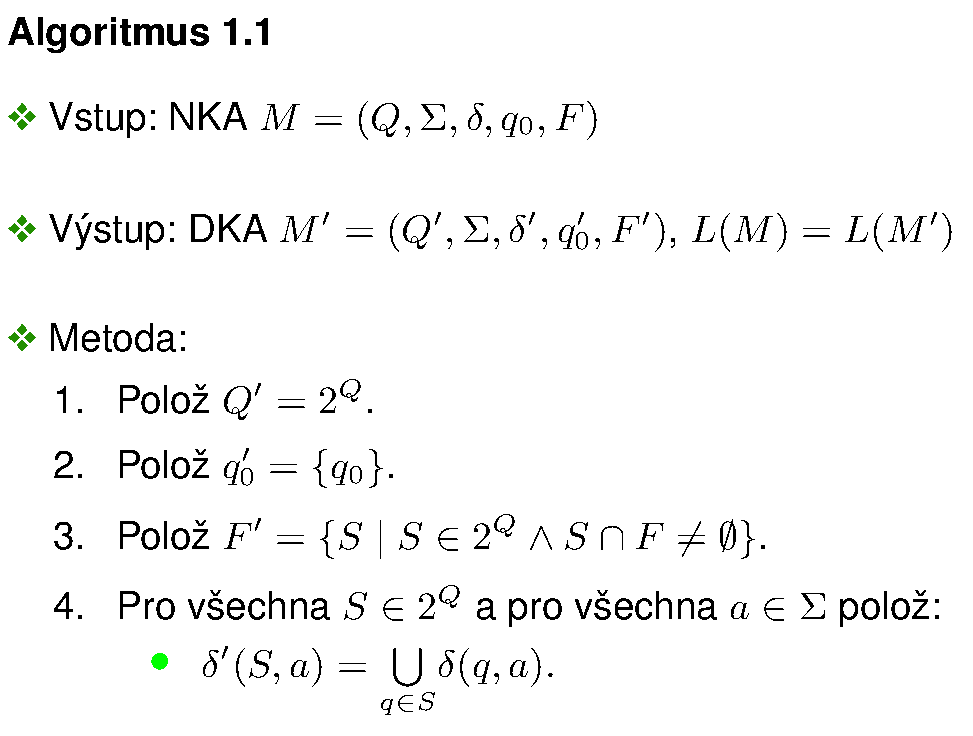
\includegraphics[width=0.7\linewidth]{nka_to_dka.pdf}
    \caption{Algoritmus determinizace NKA.}
\end{figure}

\subsection*{Příklad}

\begin{figure}[H]
    \centering
    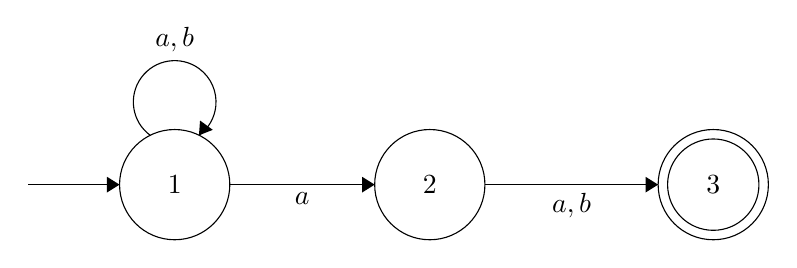
\begin{tikzpicture}[scale=0.2]
        \tikzstyle{every node}+=[inner sep=0pt]
        \draw [black] (20.6,-24.9) circle (3.5);
        \draw (20.6,-24.9) node {$1$};
        \draw [black] (36.8,-24.9) circle (3.5);
        \draw (36.8,-24.9) node {$2$};
        \draw [black] (54.8,-24.9) circle (3.5);
        \draw (54.8,-24.9) node {$3$};
        \draw [black] (54.8,-24.9) circle (2.9);
        \draw [black] (11.3,-24.9) -- (17.1,-24.9);
        \fill [black] (17.1,-24.9) -- (16.3,-24.4) -- (16.3,-25.4);
        \draw [black] (19.057,-21.774) arc (234:-54:2.625);
        \draw (20.6,-16.53) node [above] {$a,b$};
        \fill [black] (22.14,-21.77) -- (23.02,-21.42) -- (22.21,-20.83);
        \draw [black] (24.1,-24.9) -- (33.3,-24.9);
        \fill [black] (33.3,-24.9) -- (32.5,-24.4) -- (32.5,-25.4);
        \draw (28.7,-25.4) node [below] {$a$};
        \draw [black] (40.3,-24.9) -- (51.3,-24.9);
        \fill [black] (51.3,-24.9) -- (50.5,-24.4) -- (50.5,-25.4);
        \draw (45.8,-25.4) node [below] {$a,b$};
    \end{tikzpicture}
    \caption{Nedeterministický konečný automat $M$.}
\end{figure}

\begin{figure}[H]
    \centering
    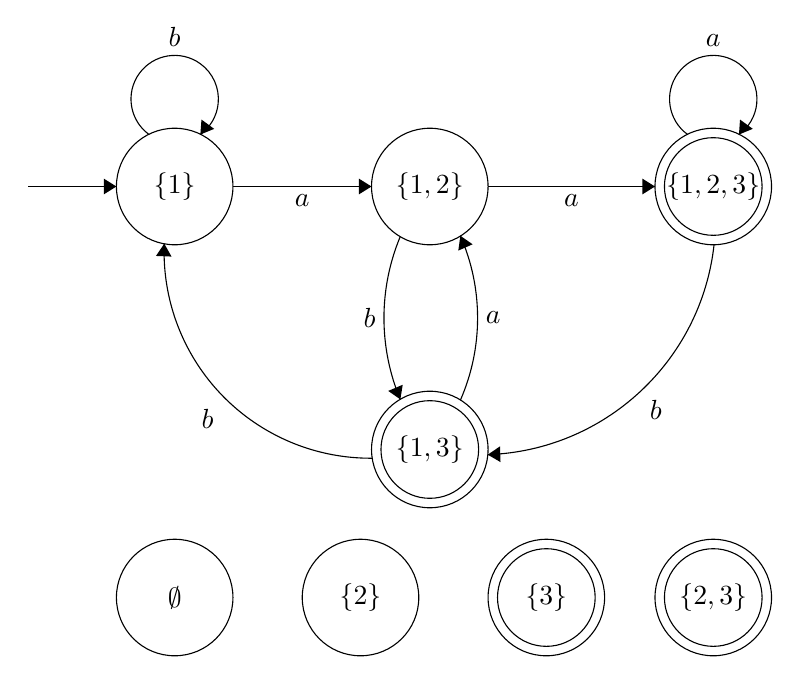
\begin{tikzpicture}[scale=0.2]
        \tikzstyle{every node}+=[inner sep=0pt]
        \draw [black] (20.7,-24.9) circle (3.7);
        \draw (20.7,-24.9) node {$\{1\}$};
        \draw [black] (36.9,-24.9) circle (3.7);
        \draw (36.9,-24.9) node {$\{1,2\}$};
        \draw [black] (54.9,-24.9) circle (3.7);
        \draw (54.9,-24.9) node {$\{1,2,3\}$};
        \draw [black] (54.9,-24.9) circle (3.1);
        \draw [black] (36.9,-41.6) circle (3.7);
        \draw (36.9,-41.6) node {$\{1,3\}$};
        \draw [black] (36.9,-41.6) circle (3.1);
        \draw [black] (20.7,-51) circle (3.7);
        \draw (20.7,-51) node {$\emptyset$};
        \draw [black] (32.5,-51) circle (3.7);
        \draw (32.5,-51) node {$\{2\}$};
        \draw [black] (44.3,-51) circle (3.7);
        \draw (44.3,-51) node {$\{3\}$};
        \draw [black] (44.3,-51) circle (3.1);
        \draw [black] (54.9,-51) circle (3.7);
        \draw (54.9,-51) node {$\{2,3\}$};
        \draw [black] (54.9,-51) circle (3.1);
        \draw [black] (11.4,-24.9) -- (17,-24.9);
        \fill [black] (17,-24.9) -- (16.2,-24.4) -- (16.2,-25.4);
        \draw [black] (19.069,-21.595) arc (234:-54:2.775);
        \draw (20.7,-16.07) node [above] {$b$};
        \fill [black] (22.33,-21.6) -- (23.21,-21.24) -- (22.4,-20.65);
        \draw [black] (24.4,-24.9) -- (33.2,-24.9);
        \fill [black] (33.2,-24.9) -- (32.4,-24.4) -- (32.4,-25.4);
        \draw (28.8,-25.4) node [below] {$a$};
        \draw [black] (40.6,-24.9) -- (51.2,-24.9);
        \fill [black] (51.2,-24.9) -- (50.4,-24.4) -- (50.4,-25.4);
        \draw (45.9,-25.4) node [below] {$a$};
        \draw [black] (33.254,-42.153) arc (-89.46343:-182.27795:13.105);
        \fill [black] (20.04,-28.53) -- (19.51,-29.31) -- (20.5,-29.35);
        \draw (23.2,-39.65) node [left] {$b$};
        \draw [black] (35.025,-38.424) arc (-157.34238:-202.65762:13.43);
        \fill [black] (35.03,-38.42) -- (35.18,-37.49) -- (34.26,-37.88);
        \draw (33.49,-33.25) node [left] {$b$};
        \draw [black] (38.843,-28.034) arc (23.64529:-23.64529:13.005);
        \fill [black] (38.84,-28.03) -- (38.71,-28.97) -- (39.62,-28.57);
        \draw (40.43,-33.25) node [right] {$a$};
        \draw [black] (54.951,-28.59) arc (-6.27863:-88.01242:14.985);
        \fill [black] (40.58,-41.93) -- (41.39,-42.4) -- (41.36,-41.4);
        \draw (51.26,-38.42) node [below] {$b$};
        \draw [black] (53.269,-21.595) arc (234:-54:2.775);
        \draw (54.9,-16.07) node [above] {$a$};
        \fill [black] (56.53,-21.6) -- (57.41,-21.24) -- (56.6,-20.65);
    \end{tikzpicture}
    \caption{Deterministický konečný automat $M'$, $L(M) = L(M')$.}
\end{figure}

%%%%%%%%%%%%%%%%%%%%%%%%%%%%%%%%%%%%%%%%%%%%%%%%%%%%%%%%%%%%%%%%%%%%%%%%%%%%%%%%

\section{Minimalizace konečného automatu}

\begin{compactitem}
    \item Proč? Zrychlení vykonávání konečného automatu.
    \item Jak? Odstraněním nepotřebných přechodů a zmenšením počtu stavů.
    \item Postup (předpokládá DKA): \begin{compactenum}
        \item Odstranění nedosažitelných stavů.
        \item Převod DKA na úplně definovaný DKA.
        \item Převod úplně definovaný DKA na redukovaný DKA (odstranění nerozlišitelných stavů).
        \item Odstranění \textit{sink} stavu.
    \end{compactenum}
\end{compactitem}

\begin{figure}[H]
    \centering
    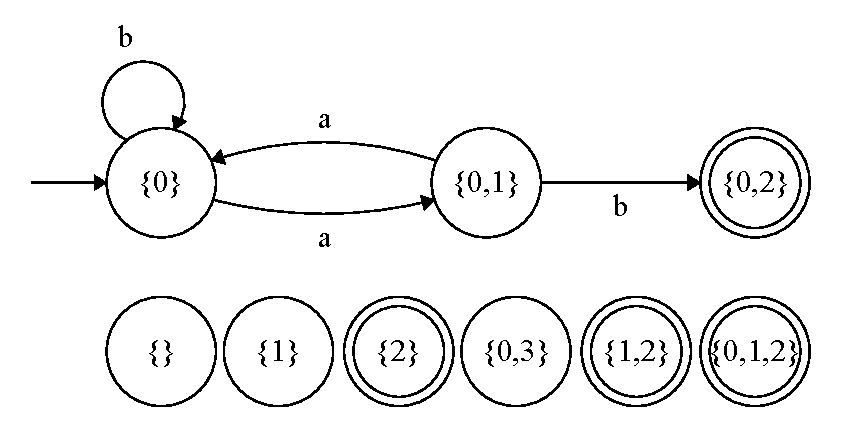
\includegraphics[width=0.75\linewidth]{dka_uplny.pdf}
    \caption{Deterministický konečný automat.}
\end{figure}

\subsection{Eliminace nedosažitelných stavů}

\begin{figure}[H]
    \centering
    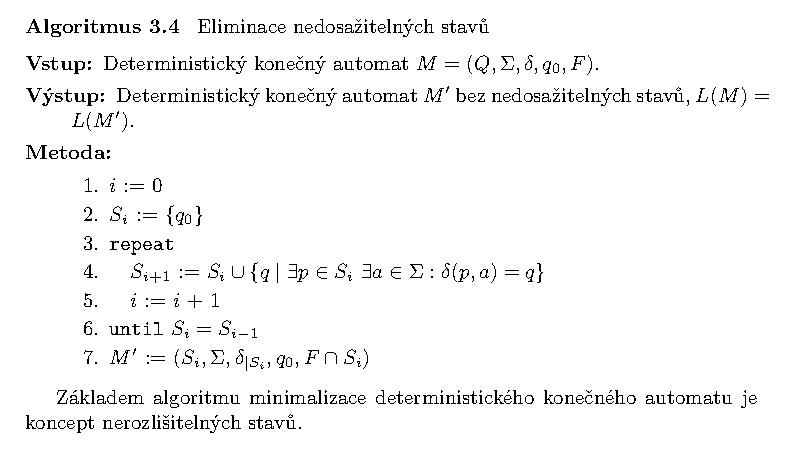
\includegraphics[width=0.9\linewidth]{eliminace_nedosazitelnych_stavu.pdf}
    \caption{Algoritmus eliminace nedosažitelných stavů.}
\end{figure}

\begin{figure}[H]
    \centering
    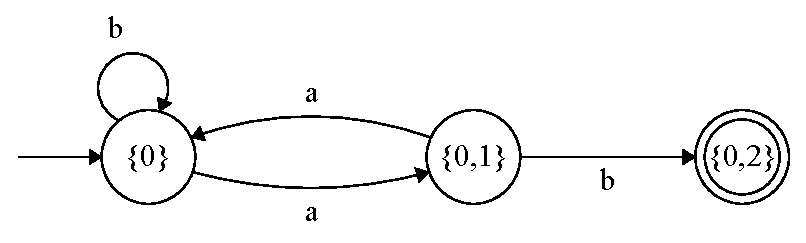
\includegraphics[width=0.75\linewidth]{dka.pdf}
    \caption{Deterministický konečný automat bez nedosažitelných stavů.}
\end{figure}

\subsection{Převod DKA na úplně definovaný}

\begin{compactitem}
    \item Vstup: DKA $M = (Q, \Sigma, \delta, q_0, F)$
    \item Výstup: úplně definovaný DKA $M'$
    \item Metoda: \begin{compactenum}
        \item $\forall q \in Q ~ \forall a \in \Sigma : \delta(q, a) = \emptyset \Rightarrow \delta'(q, a) = q_s$
        \item $\forall a \in \Sigma : \delta'(q_s, a) = q_s$
        \item $M' = (Q \cup \{ q_s \}, \Sigma, \delta \cup \delta', q_o, F)$
    \end{compactenum}
    \item $q_s$ je tzv. \textit{sink} stav.
\end{compactitem}

\begin{figure}[H]
    \centering
    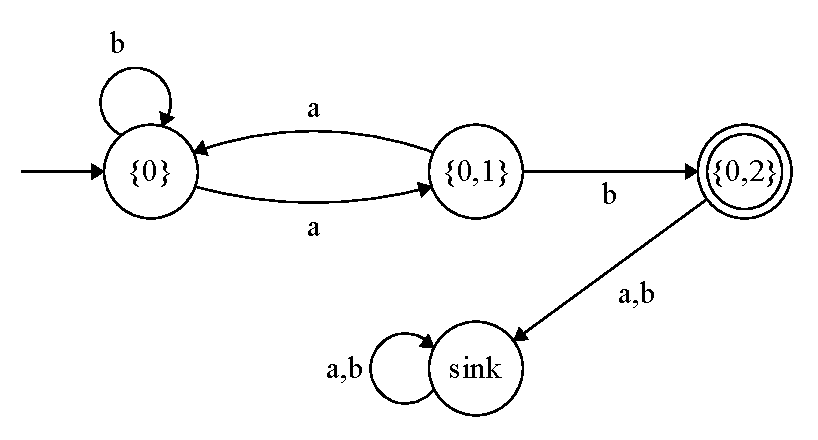
\includegraphics[width=0.75\linewidth]{dka_uplny_sink.pdf}
    \caption{Úplně definovaný deterministický konečný automat.}
\end{figure}

\subsection{Převod úplně definovaného DKA na redukovaný}

\begin{figure}[H]
    \centering
    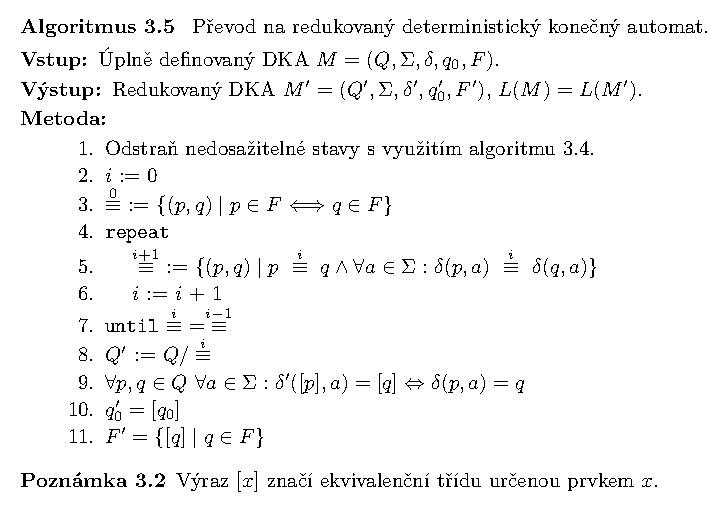
\includegraphics[width=0.9\linewidth]{prevod_na_redukovany_dka.pdf}
    \caption{Algoritmus převodu úplně definovaného DKA na redukovaný.}
\end{figure}

\subsection{Odstranění \textit{sink} stavu}

\begin{compactitem}
    \item Vstup: DKA $M = (Q, \Sigma, \delta, q_0, F)$
    \item Výstup: DKA $M'$ bez \textit{sink} stavu
    \item Metoda: \begin{compactenum}
        \item $Q' = \{ q ~|~ q \in Q \land w \in \Sigma^* \land q_f \in F \land (q, w) \vdash^* (q_f, \epsilon) \}$
        \item $\delta' = \{ (p, a, q) ~|~ \delta(p, a) = q \land q \not\in Q - Q' \}$
        \item $M' = \{ Q', \Sigma, \delta', q_0, F \}$
    \end{compactenum}
\end{compactitem}

\begin{figure}[H]
    \centering
    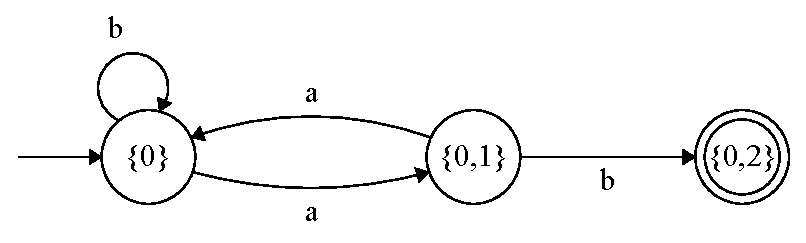
\includegraphics[width=0.75\linewidth]{dka.pdf}
    \caption{Úplně definovaný deterministický konečný automat bez \textit{sink} stavu.}
\end{figure}

%%%%%%%%%%%%%%%%%%%%%%%%%%%%%%%%%%%%%%%%%%%%%%%%%%%%%%%%%%%%%%%%%%%%%%%%%%%%%%%%

\section{Myhill-Nerodova věta}

\paragraph*{Pumping Lemma} Pumping Lemma poskytuje nutnou podmínku, ale nikoliv dostačující pro regulární jazyky, tj. když jazyk je regulární, tak podmínka musí platit. To znamená, že pomocí PL můžeme dokázat, že jazyk není regulární. Ale nemůžeme použít PL k důkazu regularity jazyky. Myšlenka Pumping Lemma spočívá v tom, že pokud mám $w \in L$, jehož délka je větší, než je počet stavů KA, který daný jazyk přijímá, tak tam musí být někde smyčka. A tím pádem, můžu tu smyčku buď úplně vypustit a nebo zopakovat vícekrát.

\paragraph*{Mihill-Nerodova věta -- kontext} Mihill-Nerodova věta charakterizuje jazyky nad $\Sigma^*$ a jejich vztah ke konečným automatům. Je silnější než Pumping Lemma, protože poskytuje nutné a dosačující podmínky pro to, aby jazyk byl regulární. Pomocí ní můžeme dokázat, že jazyk je a nebo není regulární.

\paragraph*{Relace ekvivalence} Relace ekvivalence je binární relace (značíme $\thicksim$), která je reflexivní, symetrická a tranzitivní. Rozkládá množinu nad kterou je definovaná na tzv. \textbf{třídy ekvivalence}. Pro každé dvojice tříd ekvivalence platí, že jsou vzájemně disjunktní. Sloučením všech tříd ekvivalence dostaneme původní množinu. Počet tříd rozkladu je tzv. \textbf{index ekvivalence}. Tříd může být i nekonečno, pak index definujeme jako $\infty$. Relaci ekvivalence nad množinou $\Sigma^*$ zapisujeme jako $\Sigma^* / \thicksim$.

\paragraph*{Pravá kongruence} Pravá kongruence (pravá invariance) je speciální typ relace ekvivalence, která splňuje požadovanou vlatnost. Nechť $\Sigma$ je abeceda a $\thicksim$ je relace ekvivalence nad $\Sigma^*$. Relace ekvivalence $\thicksim$ je pravou kongruencí pokud platí: $$ \forall u, v, w \in \Sigma^* ~:~ u \thicksim v \Rightarrow uw \thicksim vw $$
Myšlenka: Pro všechny slova $u, v$ z jazyka platí, že pokud jsem se přes ně dostal do nějakého (stejného) stavu, tak když k oboum připojím slovo $w$, tak se zase dostanu do stejného stavu.

\paragraph*{Prefixová ekvivalence} Nechť $L$ je libovolný (ne nutně regulární) jazyk nad abecedou $\Sigma$. Na množině $\Sigma^*$ definujeme relaci $\thicksim_L$ zvanou prefixová ekvivalence pro $L$ takto: $$ u \thicksim_L v \Leftrightarrow ( \forall w \in \Sigma^* ~:~ uw \in L \Leftrightarrow uw \not\in L )$$
Myšlenka: slova $u$ a $v$ dovedou konečný automat do stejného stavu.

\paragraph*{Mihill-Nerodova věta} Jazyk $L \subseteq \Sigma^*$ je regulární právě když: \begin{compactitem}
    \item $\exists \text{KA} ~ M : L(M) = L$
    \item Existuje pravá kongruence $\thicksim$ konečného indexu na $\Sigma^*$ taková, že $L$ je sjednocením vybraných tříd rozkladu $\Sigma^* / \thicksim$.
    \item Relace prefixové ekvivalence $\thicksim_L$ má konečný index (existuje minimální KA, který odpovídá).
\end{compactitem}

Pokud dokážu, že nad daným jazykem neexistuje relace pravé kongruence s konečným indexem, tak jazyk není regulární.
